\newpage
\setcounter{page}{11}
\section{Обработка результатов измерений}

Приводим графики полученных спектров:

\begin{figure}[h!]
	\centering{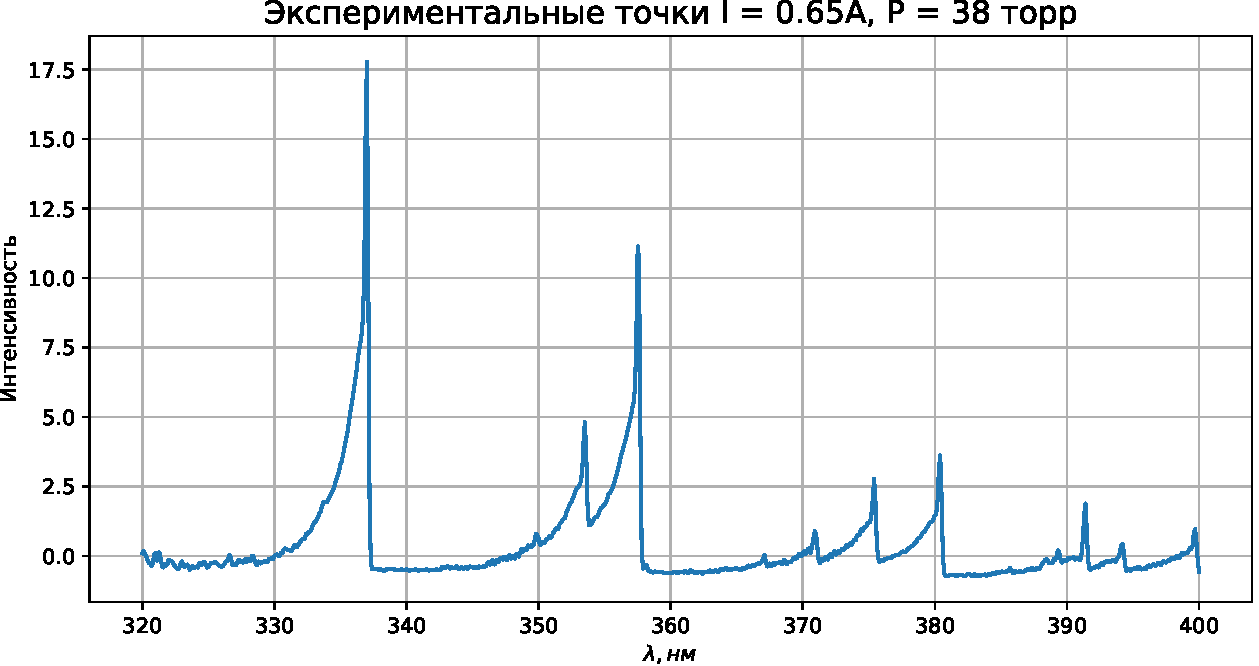
\includegraphics[scale=0.6]{p1.pdf}}
	\label{fig:image}
\end{figure}

\begin{figure}[h!]
	\centering{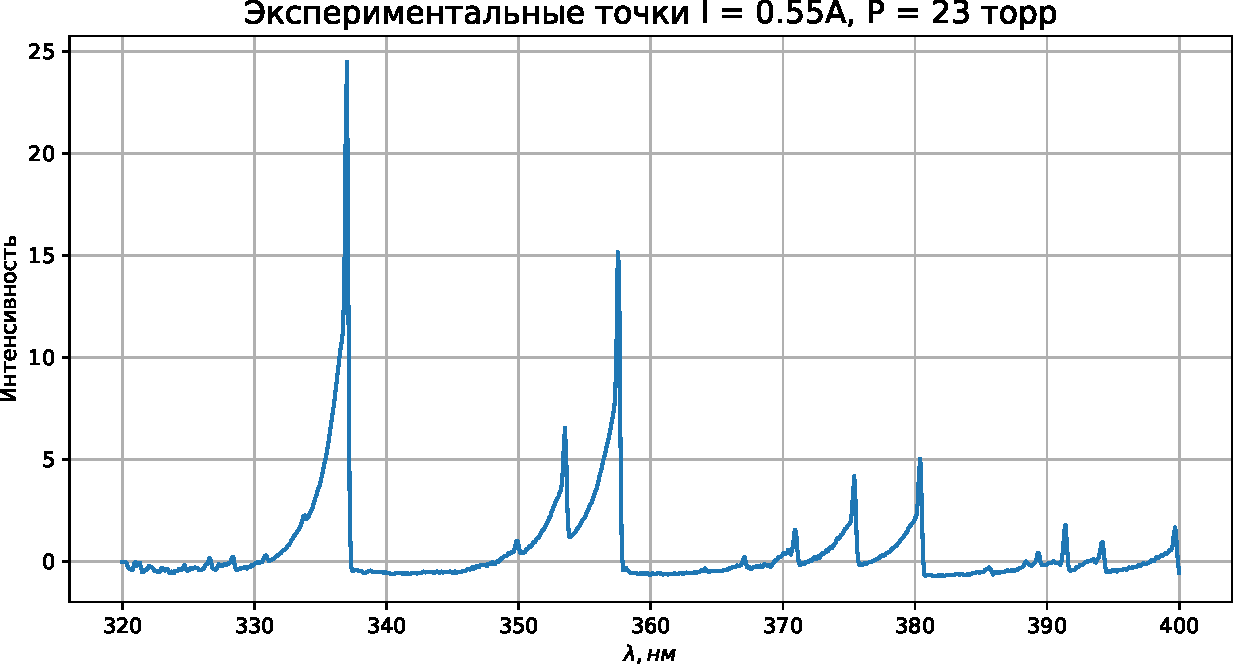
\includegraphics[scale=0.6]{p4.pdf}}
	\label{fig:image}
\end{figure}

\begin{figure}[h!]
	\centering{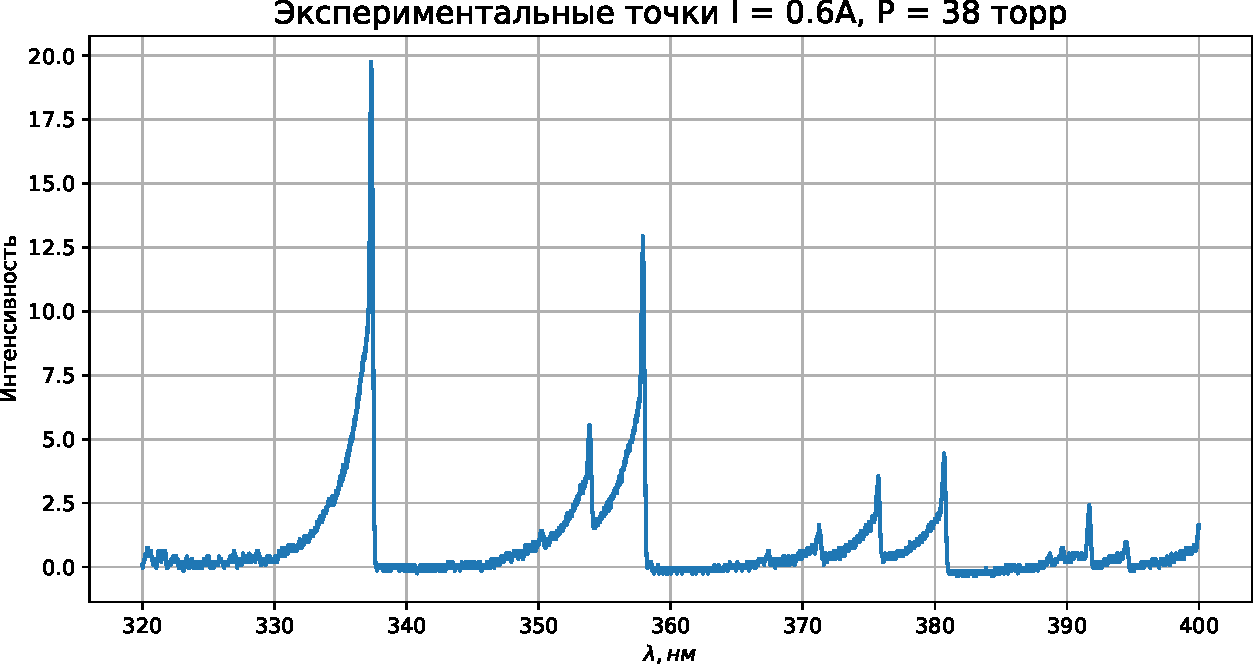
\includegraphics[scale=0.6]{p2.pdf}}
	\label{fig:image}
\end{figure}

Далее проводим сравнения положения полученных пиков, соответствующих одним переходам:
Это требуется в связи с особенностью установки. Шкала по длине волны в ходе эксперимента 
могла сдвинуться.

\begin{figure}[h!]
	\centering{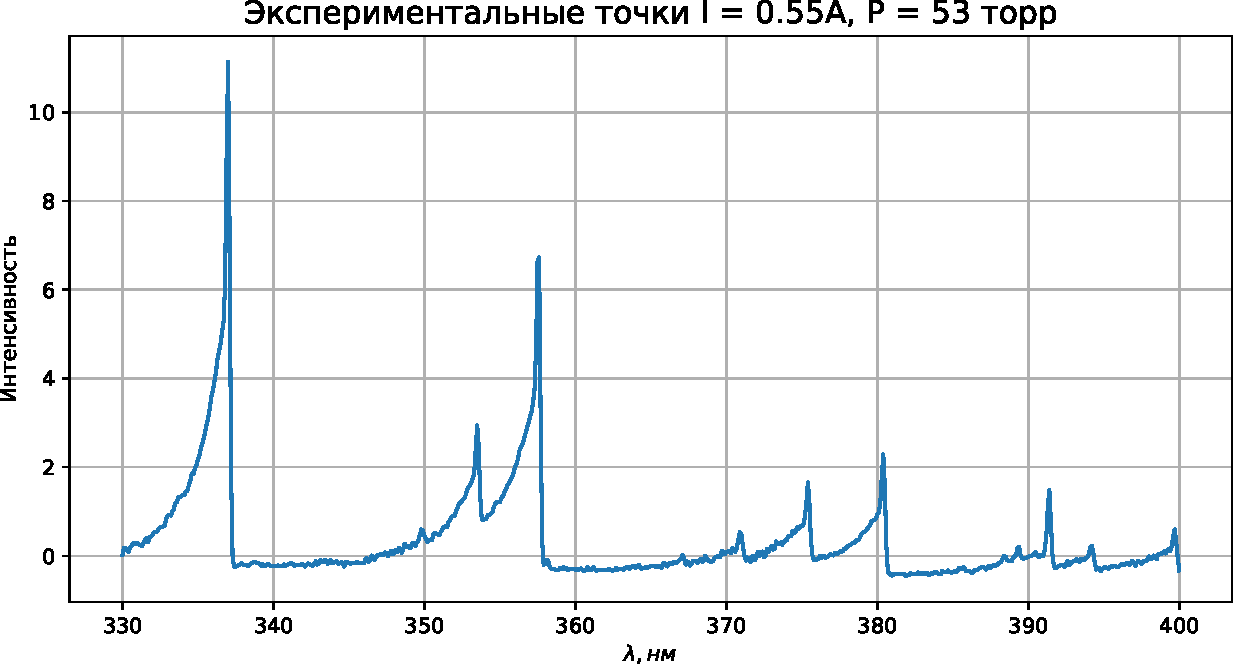
\includegraphics[scale=0.6]{p3.pdf}}
	\label{fig:image}
\end{figure}

\begin{figure}[h!]
	\centering{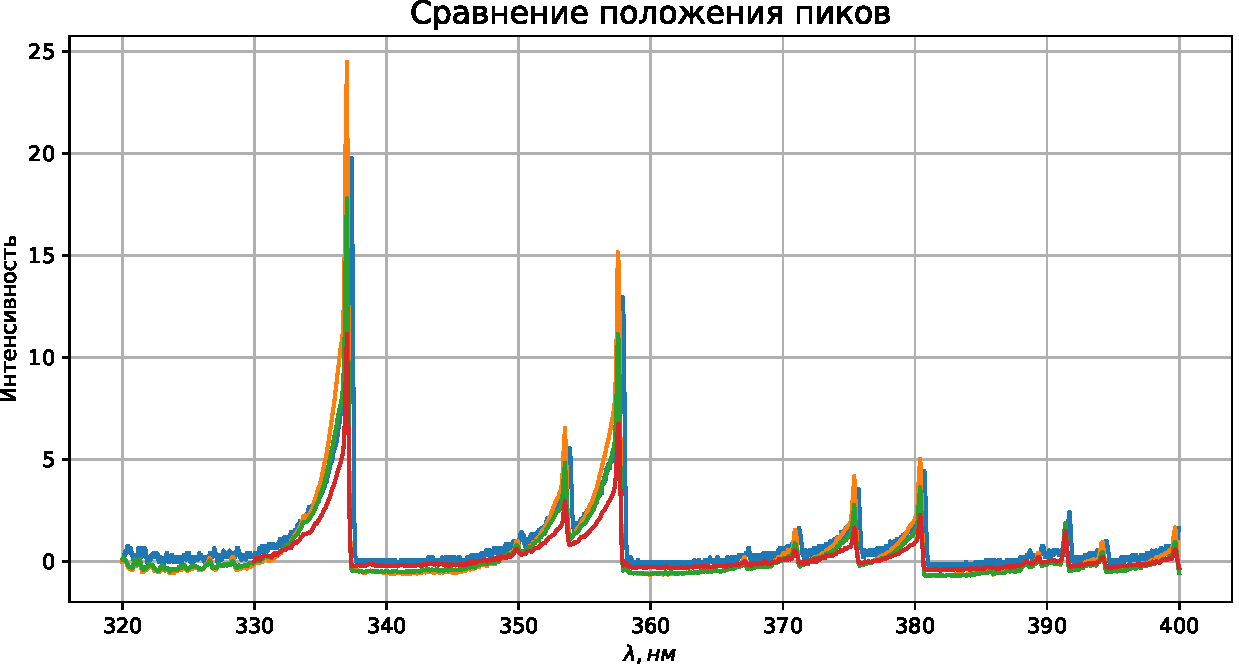
\includegraphics[scale=0.6]{p5.pdf}}
	\label{fig:image}
\end{figure}

\begin{figure}[h!]
	\centering{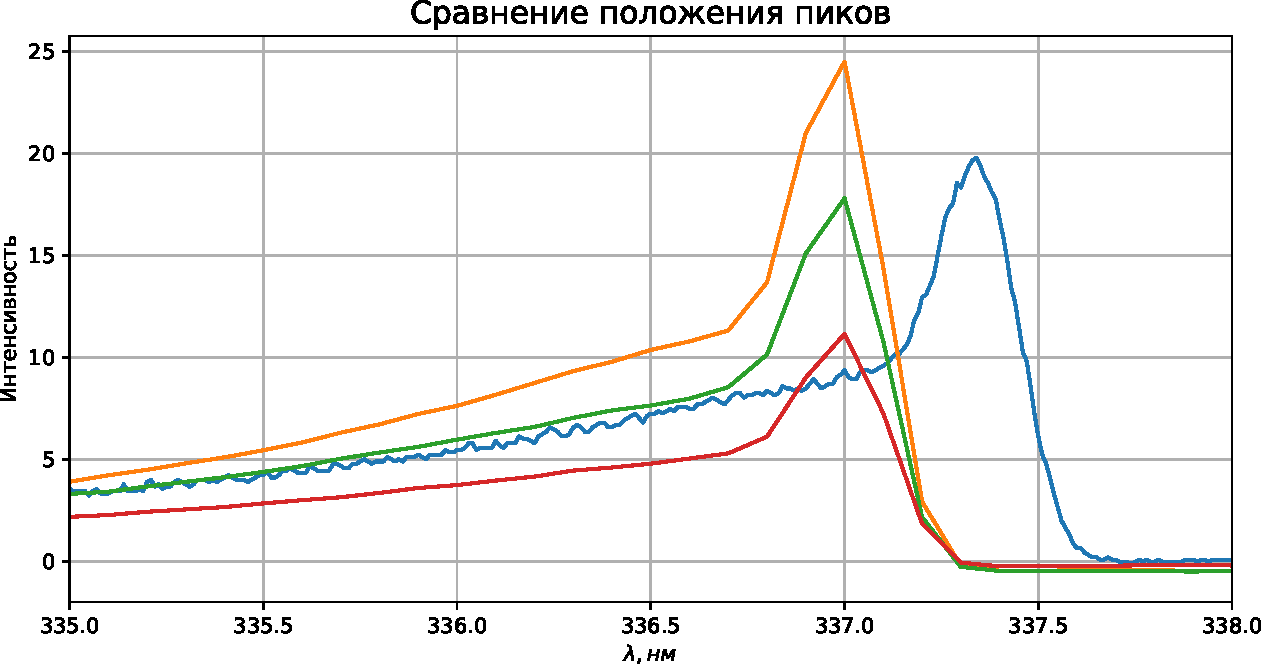
\includegraphics[scale=0.6]{p6.pdf}}
	\label{fig:image}
\end{figure}

Проведем идентификацию и соотнесение наблюдаемых полос:

\begin{table}[h!]
	\begin{tabular}{|l|l|l|l|l|l|l|l|l|l|}
		\hline
		Переход $\nu^{\prime}  \rightarrow \nu^{\prime \prime}  $    & 0$\rightarrow$0  & 2$\rightarrow$3  & 1$\rightarrow$2  & 0$\rightarrow$1  & 2$\rightarrow$4  & 0$\rightarrow$2  & 2$\rightarrow$5  & 1$\rightarrow$4  & 1$\rightarrow$3  \\ \hline
		Длина волны, A & 3370 & 3499 & 3535 & 3575 & 3709 & 3804 & 3942 & 3997 & 3754 \\ \hline
	\end{tabular}
\end{table}

\newpage

\subsection{Вычисление вращательной температуры:}

Для вычисления вращательной температуры выберем участок неразрешенной вращательной
структуры и прологарифмируем его. По наклону прямой зависимости $lg(I) = f(\lambda)$ , используя
рассчитанную зависимость тангенса угла наклона от значения вращательной температуры, определим значение вращательной температуры в центральной части разряда.

\begin{figure}[h!]
	\centering{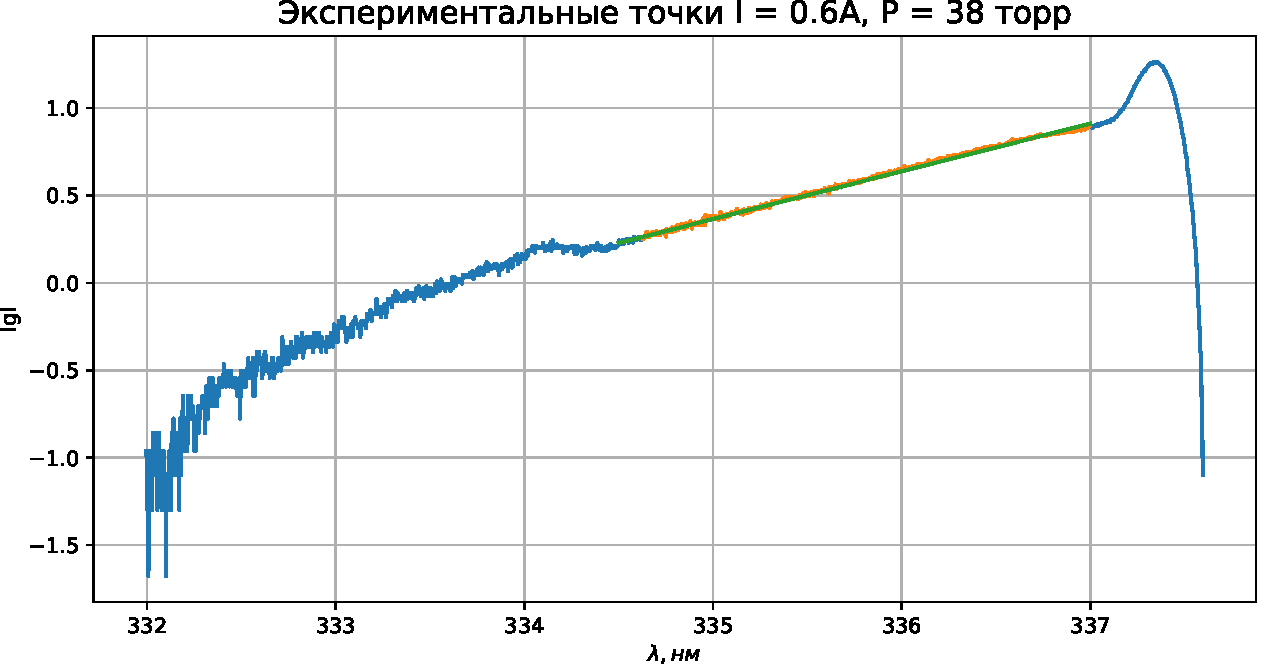
\includegraphics[scale=0.8]{p7.pdf}}
	\label{fig:image}
\end{figure}

\begin{figure}[h!]
	\centering{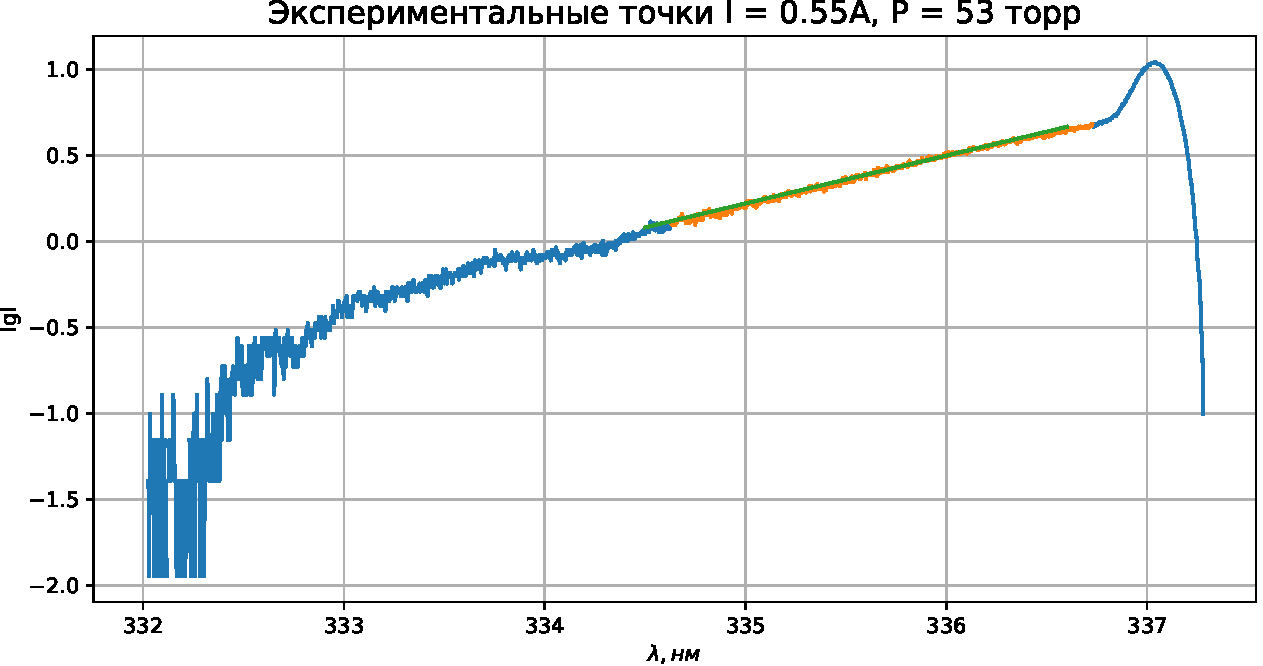
\includegraphics[scale=0.8]{p8.pdf}}
	\label{fig:image}
\end{figure}

\begin{figure}[h!]
	\centering{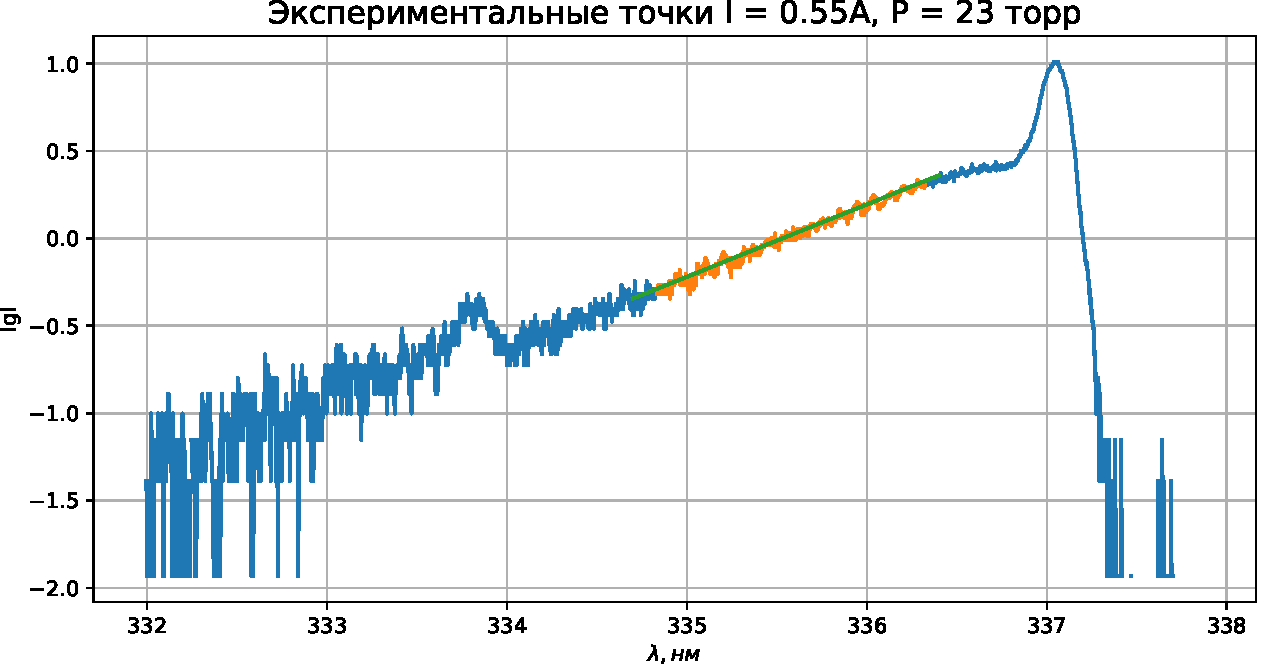
\includegraphics[scale=0.8]{p9.pdf}}
	\label{fig:image}
\end{figure}

Привожу полученные значения вращательных температур для представленных зависимостей:

\begin{displaymath}
T_{1,2} \approx 1300\hspace{2mm} K,\hspace{2mm}T_3 \approx 1000\hspace{2mm}K
\end{displaymath}

\subsection{Определение колебательной температуры:}

По спектрам полос $0 \rightarrow 1$,$\hspace{2mm} 1\rightarrow 2$,$\hspace{2mm} 2\rightarrow 3$ и $ \hspace{2mm} 0\rightarrow 2$, $ \hspace{2mm} 1\rightarrow 3$,$ \hspace{2mm} 2\rightarrow 4$
определим колебательную
температуру в центральной части разряда и в приэлектродных областях, используя соотношение:

\begin{displaymath}
ln(\frac{I_{\nu^{\prime}\nu^{\prime \prime}}}{\nu^4_{\nu^{\prime}\nu^{\prime \prime}}q_{\nu^{\prime}\nu^{\prime \prime}}}) = -\frac{G(\nu^{\prime})}{0.6925T_{vib}}+C
\end{displaymath}

Найдем интенсивности пиков:

\begin{figure}[h!]
	\centering{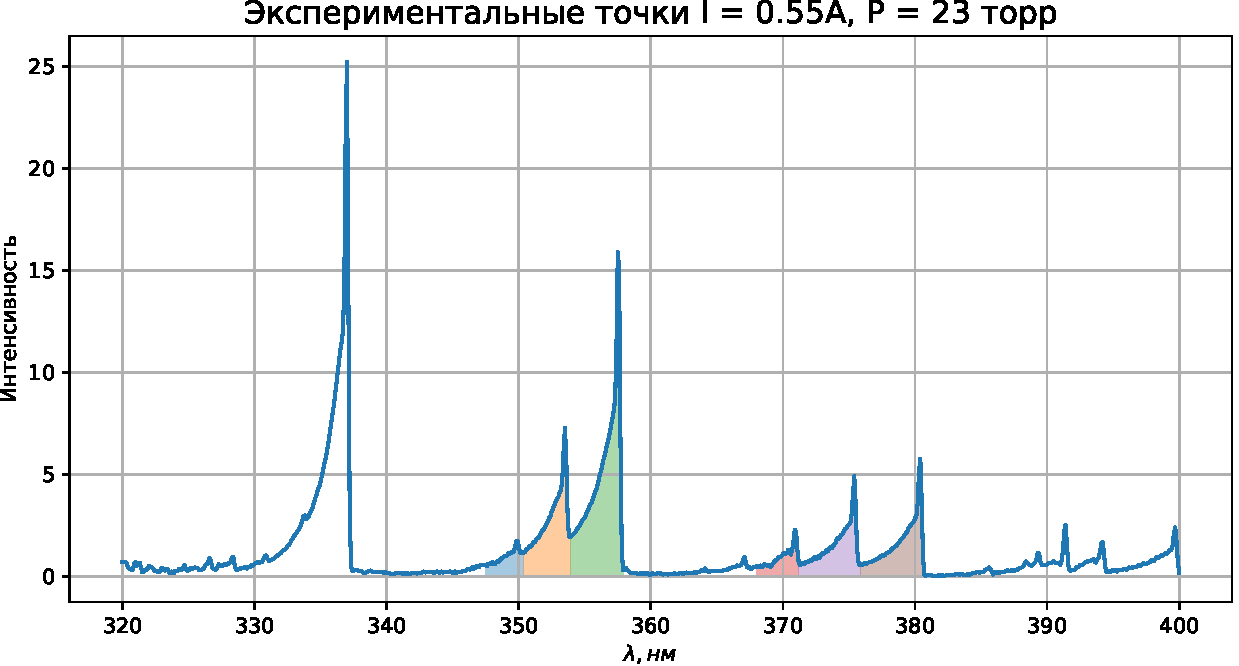
\includegraphics[scale=0.8]{p10.pdf}}
	\label{fig:image}
\end{figure}

\begin{displaymath}
S23 =  2.85;\hspace{2mm}
S12 =  9.83;\hspace{2mm}
S01 =  19.71;\hspace{2mm}
S24 =  2.92;\hspace{2mm}
S13 =  7.06;\hspace{2mm}
S02 =  7.8
\end{displaymath}

\newpage

Итак, построим необходимую зависимость для двух серий:

\begin{figure}[h!]
	\centering{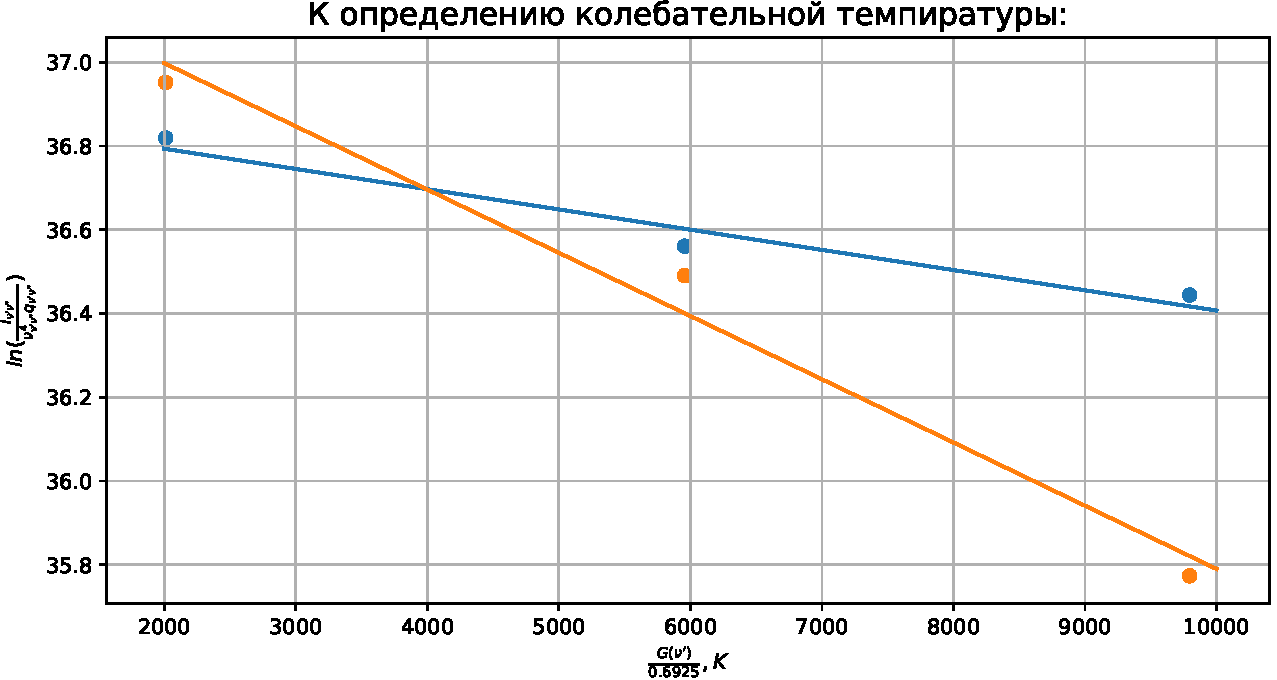
\includegraphics[scale=0.8]{p11.pdf}}
	\label{fig:image}
\end{figure}

Откуда:

\begin{displaymath}
T_{1vib} \approx 2\cdot 10^4 K \hspace{2mm} T_{2vib} \approx 6.5\cdot 10^3 K
\end{displaymath}

\subsection{Заключение}
В данной работе были получены электронно-колебательно-вращательные спектры, качественный вид которых был представлен в зависимости от внешних параметров $(P,I)$. Также были посчитаны вращательные температуры по электронно-колебательно-вращательным спектрам излучения второй положительной системы азота при разных токах и
давлениях, а так же колебательные температуры. Используемая методика нахождения этих температур даёт адекватные, но грубые результаты. Оказалось, что при повышении
давления в газе вращательная температура увеличивается. Также видно, что в представленной неравновесной системе колебательная температура значительно превосходит вращательную.